\begin{block}{What is Mezuro?}
    \begin{figure}
        \begin{center}
            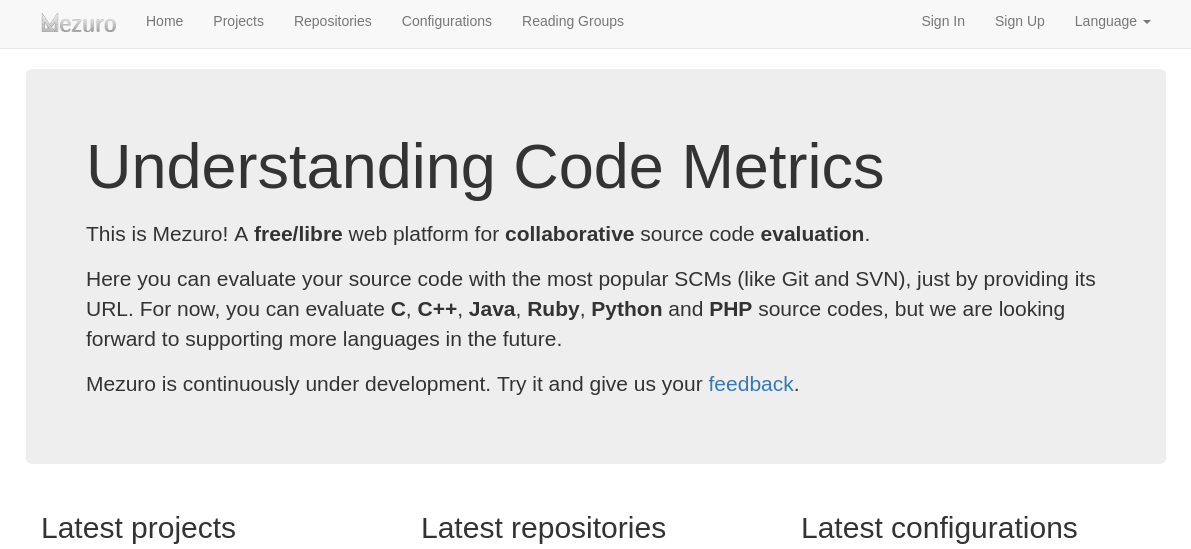
\includegraphics[width=\textwidth]{figures/MezuroHome.png}
            \label{fig:feature1}
        \end{center}
    \end{figure}

    \begin{itemize}
        \item FOSS web-based platform that analyzes source code

        \item It allows developers to compare analyzed projects and share
            knowledge about metrics

        \item Goal to help software developers and maintainers to understand
            and feel comfortable using source code metrics during their projects

        \item Results are public

        \item Extensible architecture

        \item Currently supports Ruby, PHP, Java, C/C++, and Python

    \end{itemize}
\end{block}
